\section{Aktieru modelis}
\label{sec:actormodel}

Aktieru modelis apraksta veidu kā realizēt vienotu atteikumnoturīgu informācijas
sistēmu, kas sastāv no vairākām atsevišķām, paralēli darbinātām mazākām
informācijas sistēmām - aktieriem. Aktieru modelī aktieri var 1) sūtīt ziņas, 2)
izveidot jaunus \glslink{actor}{aktierus} un 3) definēt kā reaģēt uz ziņām kas
tiek adresētas tiem pašiem. \cite[p. 1]{CarlHewitt2010}

Svarīga īpatnība aktieru modelī, kas ļauj tam labi aprakstīt reālu, fizisku
infrastruktūru (kas ir svarīgi šī darba ietvaros, jo ir nepieciešams modelēt
fizisku attīstītājrīku aparatūru), ir pamatprincips, ka aktieriem piemīt laicīgs
dzīvescikls jeb jebkurā brīdī tie var sākt darboties vai beigt darboties.
\cite[p. 6]{CarlHewitt2010} 
 
Šī īpatnība ir noderīga darba ietvaros, jo fiziskā aparatūra var salūzt, zaudēt
elektrību, zaudēt interneta savienojumu, utml. Kā arī šis modelis ir vērtīgs, jo
eksistē publiski pieejami satvari, kas ir izstrādāti pēc šī modeļa un tātad ļauj
projektēt šāda veida sistēmas. Šī darba ietvaros ir izmantots satvars Akka, kas
ir pieejams Java, Scala un .NET programmēšanas valodās, taču konceptuāli līdzīgi
satvari eksistē arī daudzās citās valodās, piem. Erlang valodā OTP satvars, Rust
valodā Actix, Haskell valodā Cloud Haskell, utml.

\begin{figure}[H]
    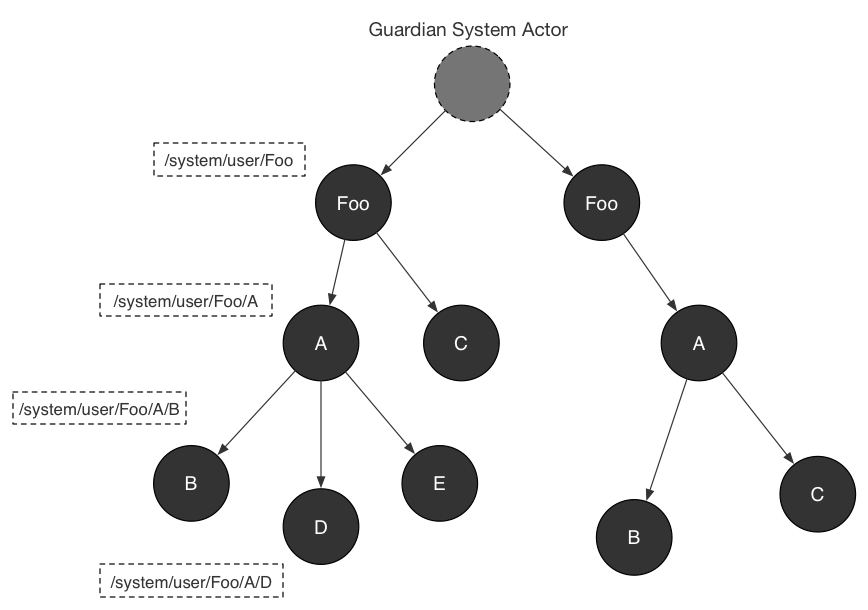
\includegraphics[width=0.5\linewidth]{assets/akka-actor-hierarchy-gray.png}
    \centering
    \caption{\glslink{actorsystem}{Aktieru modeļa sistēmas} hierarhija.
    \cite[sl. 34]{MarkusJuraAkka}}
    \label{fig:actorsystem}
\end{figure}

Attēlā \ref{fig:actorsystem} redzama aktieru modelim specifiskā aktieru sistēmas
hierarhija - kuru "bērna" aktieri izveidojis kurš "vecāka" aktieris. Aktieru
sistēmas parasti sastāv no sistēmas aktieriem un lietotāja aktieriem, parasti ir
viens saknes aizbildnības aktieris, kas izveido sistēmas un lietotāju
aizbildnības aktierus, savukārt, programmētājs izmanto šo lietotāju aizbildnības
aktieri, lai izveidotu savu biznesa loģikas saknes aktieri, kas savukārt
izveidos veselu biznesa loģikas aktieru hierarhiju atbilstoši vajadzībām.
\cite[para. The Akka actor hierarchy]{LightbendAkka2619}

\section{Notikumu sistēmas}
\label{sec:eventsourcing}

Piedāvātajā risinājumā caurvijas koncepts par notikumu sistēmām. Notikumu
sistēma ir tāda informācijas sistēma, kas apstrādā komandas jeb vēlamās izmaiņas
sistēmā, potenciāli akceptē komandas notikumos jeb veiktajās izmaiņās, izmaina
sistēmas stāvokli atbilstoši šiem notikumiem jeb  izmaiņām kā arī izpilda
blakusefektus jeb reakcijas atbilstoši šiem notikumiem, lai izmainītu kādas
ārējas sistēmas stāvokli.
\cite[para. 3.2.3]{JohnsenEspen2018}

Notikumu sistēmas pamatā ir notikumu dzinējs, kas realizē vēlamo sistēmas
loģiku. Šāds dzinējs, to mazliet abstrahējot, sastāv no trīs detaļām: 1)
stāvoklis jeb dati, kas tiek sākotnēji izveidoti un tad mainīti atbilstoši
notikumiem, 2) funkcija, kas lasa šobrīdējo stāvokli un validē komandas jeb
noraida tās vai akceptē tās notikumos un 3) funkcija, kas reaģē uz notikumiem
jeb attīsta aktuālo stāvokli jeb datus un izpilda notikumu blakusefektus. Attēlā
\ref{fig:eventengine} redzams šādas sistēmas dzīvescikls jeb stāvoklis,
validācijas un attīstības funkcijas un izpildītie blakusefekti.

Notikumu sistēmas iet roku rokā ar iepriekšminēto aktieru modeli. Katru aktieri
var realizēt kā notikumu sistēmu - 1) aktieris saņem ziņas no citiem aktieriem
jeb komandas jeb vēlamās izmaiņas, tās tiek validētas jeb akceptētas vai
noraidītas, 2) komandas rezultē akceptētos notikumos, 3) notikumi izmaina
aktuālo stāvokli un rezultē blakusefektos. 

\begin{figure}[H]
    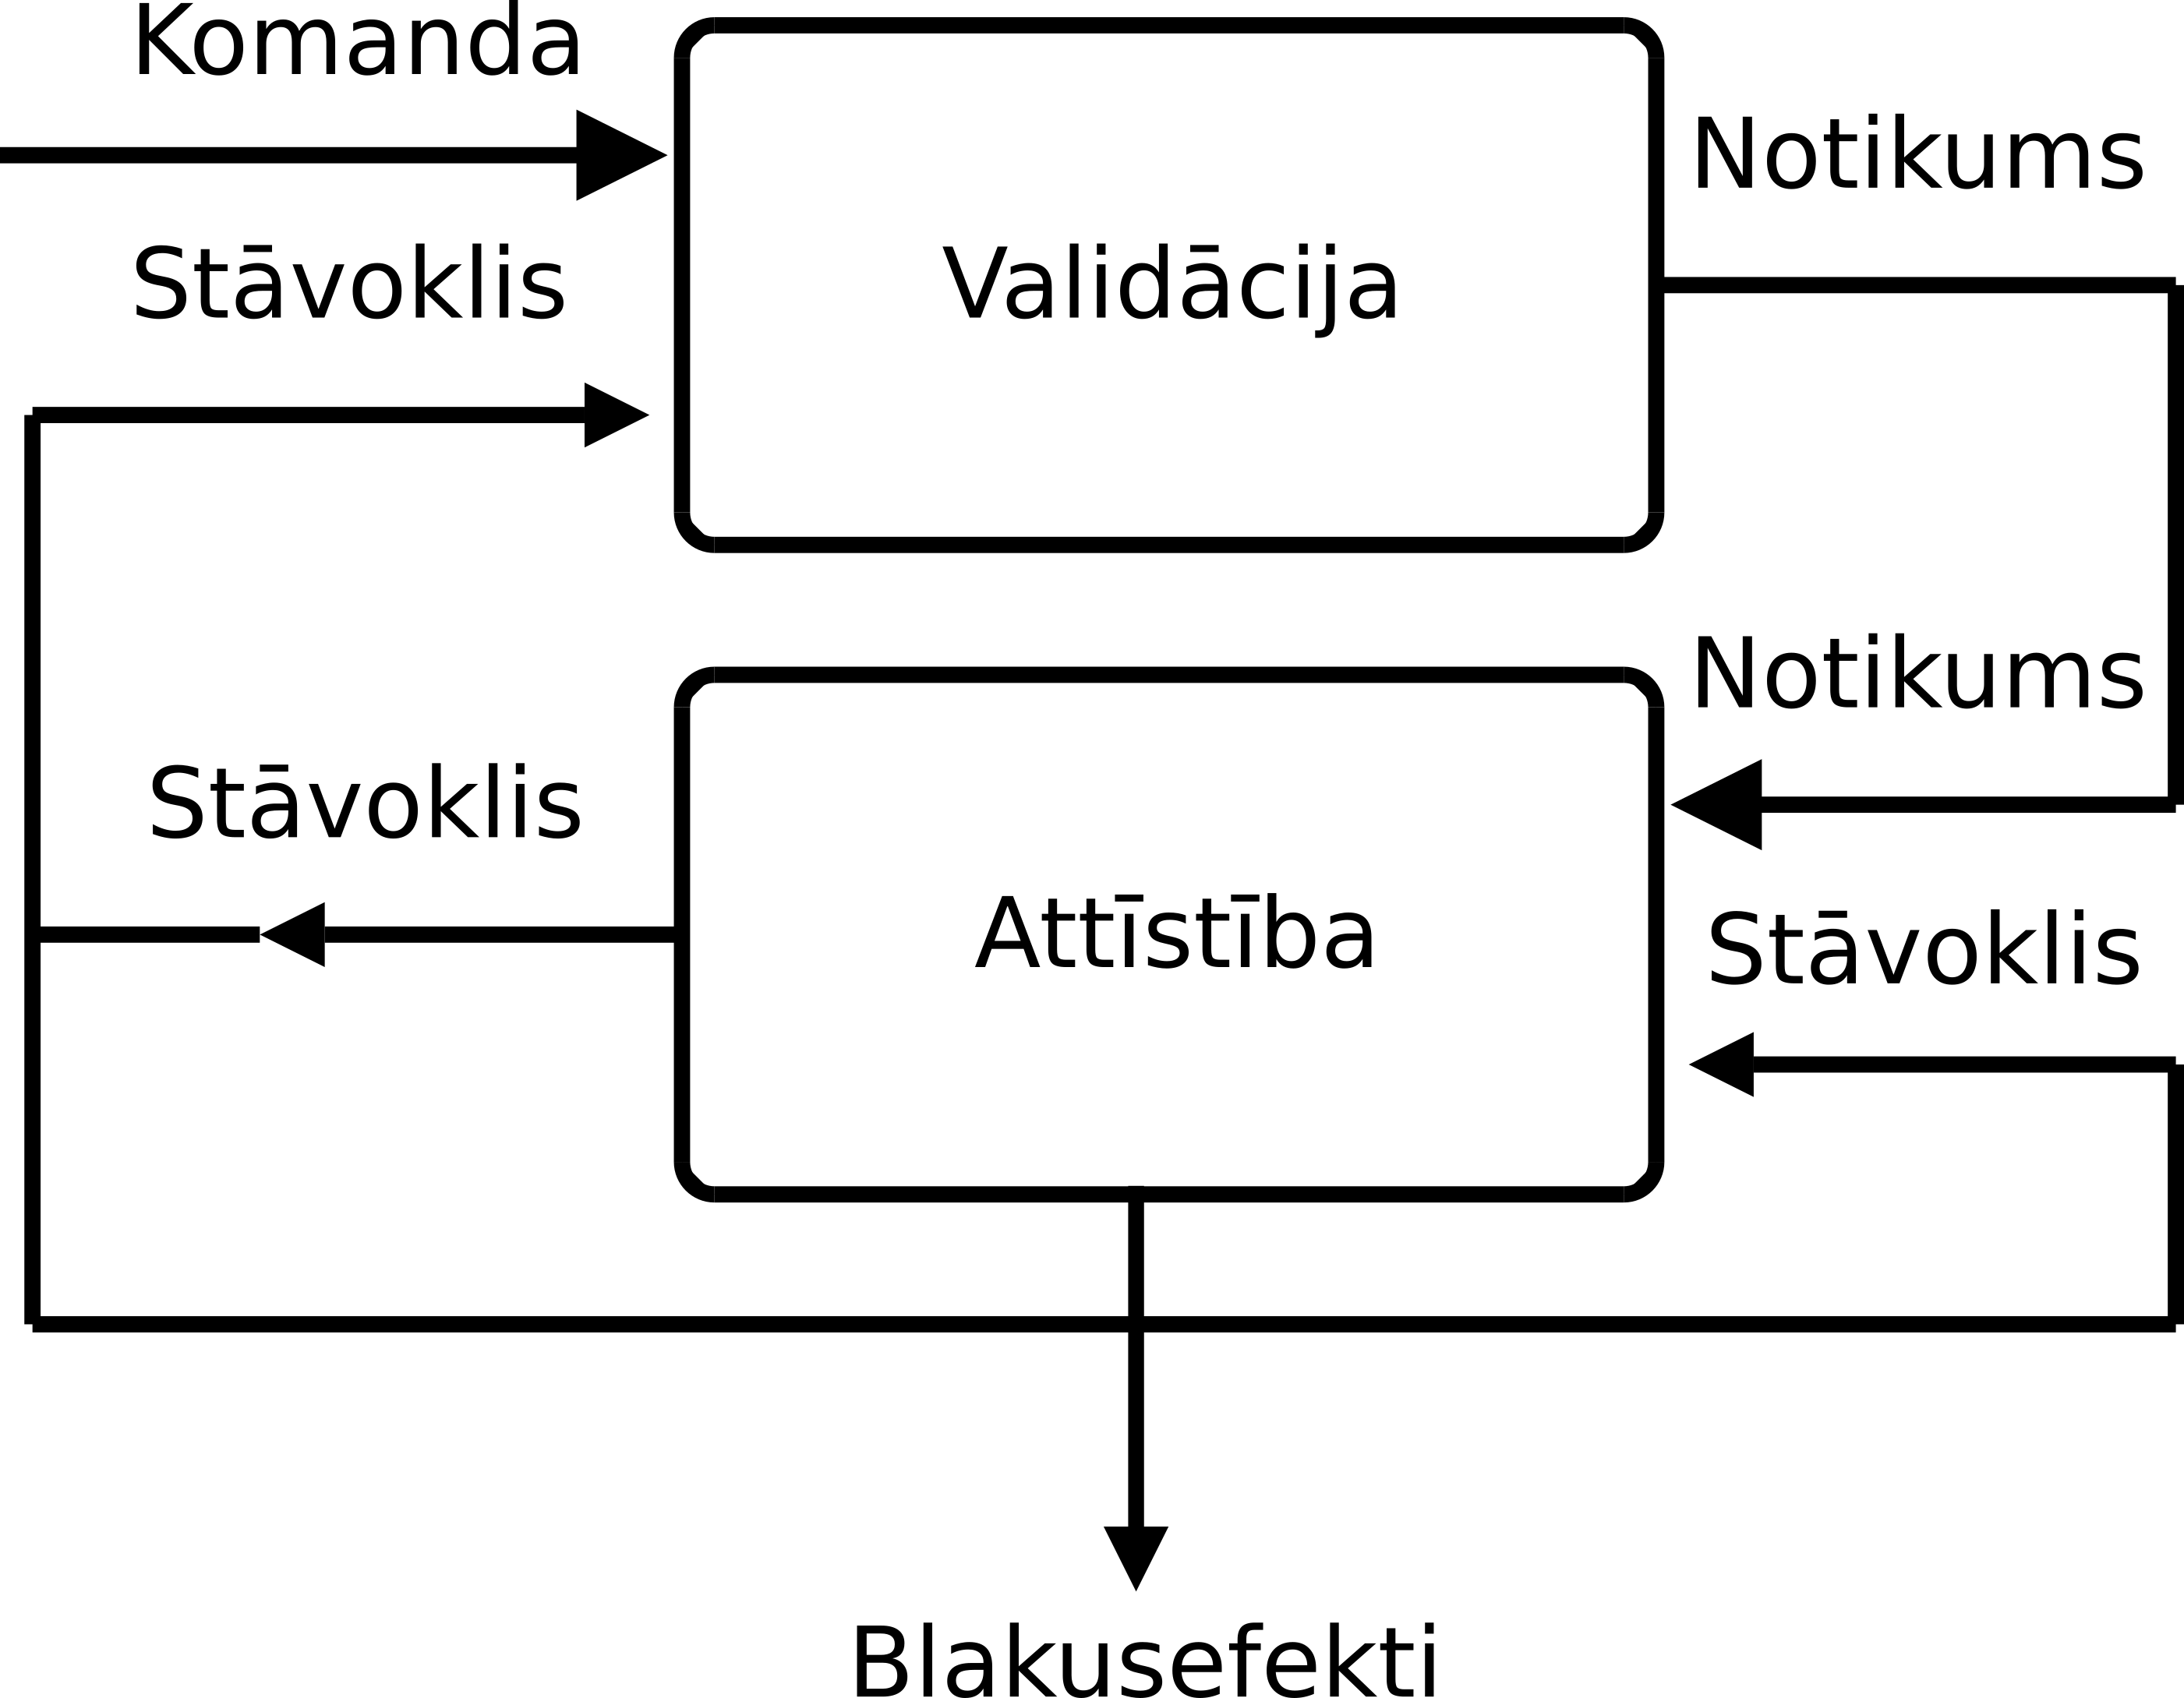
\includegraphics[width=0.5\linewidth]{assets/event-sourcing-decider.png}
    \centering
    \caption{Notikumu sistēmas apstrādes cikls. Papildināts no tiešsaistes avota. \cite{JeremieChassaing2021}}
    \label{fig:eventengine}
\end{figure}

Darba ietvaros katram attīstītājrīkam tiek piesaistīta viena vai vairākas
pārvaldības notikumu sistēmas jeb "aģenti". Aģents ir paredzēts, lai pārvaldītu
video straumēšanu, programmatūras augšupielādi, seriālā porta monitorēšanu, un
viss tiek realizēts izmantojot komandas, notikumus un blakusefektus. Tai skaitā
arī platformas lietotāji attālināti mijiedarbojoties ar attīstītājrīkiem izmanto
virtuālās saskarnes, piem. MinOS., kas arī ir realizētas kā notikumu sistēmas.
Pašā platformā, centralizētajā \glslink{server}{serverī}, lietotāju un aģentu
apkalpošanas mehānismi ir realizēti izmantojot notikumu sistēmas un aktieru
modeli. 

\section{Digitālas aparatūras projektēšana}

Lai digitalizētu mijiedarbību ar attīstītājrīku aparatūru, ir nepieciešams, lai
aparatūra ir spējīga kooperēties ar mūsu platformu, kas nozīmē, ka to ir jāprot
korekti noprogrammēt jeb, precīzāk, tajā jāaugšupielādē atbilstoši projektēta
loģisko elementu konfigurācija jeb programmaparatūra, kas nodrošinās mūsu vēlamo
mijiedarbību ar platformu.

Ir dažādi veidi kā attīstājrīka aparatūra varētu mijiedarboties ar izstrādāto
platformu, kas vēlākās nodaļās tiek arī detalizētāk apskatīti, bet pamatā ir
jāsaprot, ko īsti nozīmē digitālās aparatūras projektēšana. Digitālās aparatūras
projektēšana sevī ietver 1) signālus, 2) loģiskus elementus, 3) vadus starp tiem
loģiskajiem elementiem, 4) šo elementu izvietošanu integrētā shēmā. 

Vērtīgi pieminēt, ka loģiskie elementi šajā kontekstā nozīmē ne tikai
kombinatorās loģikas elementus, kas realizē loģikas tabulas un funkcionē bez
stāvokļa (angl. stateless), bet arī sekvenciālās loģikas elementus, kas realizē
atmiņu, piem. flip-flop. \cite[para 1.1]{LarryMassengale2018} 

\begin{figure}[H]
    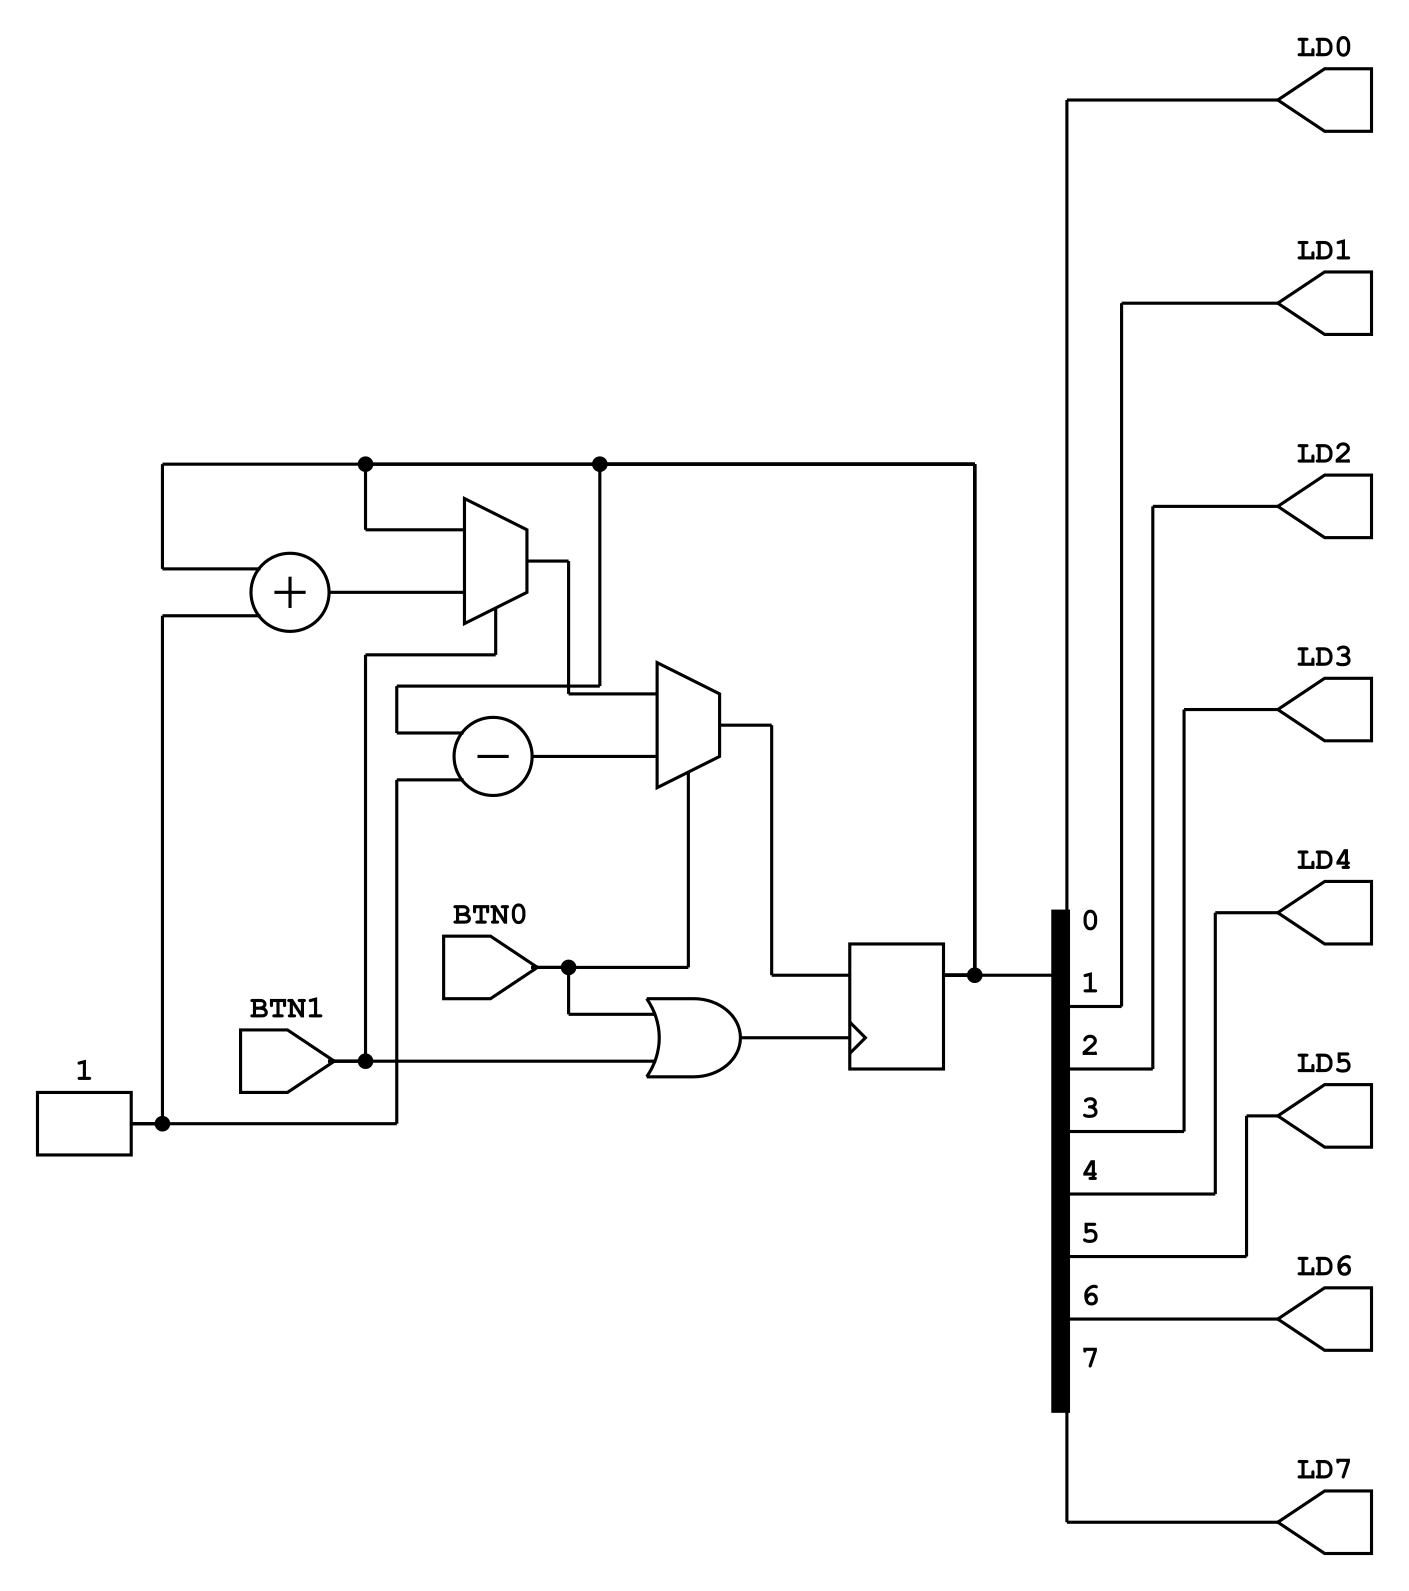
\includegraphics[width=0.5\linewidth]{assets/counter.png}
    \centering
    \caption{Loģisko elementu konfigurācija "pieskaitītājs un atņēmējs"}
    \label{fig:counter}
\end{figure}

Attēlā \ref{fig:counter} redzama tipiska loģisko elementu konfigurācija, kas
ilustrē visus iepriekšminētos projektēšanas pamatelementus. Konfigurācijā
redzami divi ievadsignāli "BTN0" un "BTN1" un astoņi "LD{0-7}" izvadsignāli.
Papildus konfigurācijā izmantots astoņu bitu atmiņas flip-flop reģistrs
(taisnstūris ar trijstūri), signālu multipleksors, kas atkarībā no "nosacījuma"
signāla ārā izvada vai nu vienu signālu vai otru (trapece), konstants astoņu
bitu signāls ar vieninieka vērtību (taisntūris ar "1"). Kad "BTN0" signāls top
no 0 par 1, reģistrā "1" tiek atņemts vieninieks. Kad "BTN1" signāls top no 0
par 1, reģistrā "0" tiek pieskaitīts vieninieks. Astoņu bitu reģistra "1" bitu
vērtība tiek izvadīta izvadsignālos "LD{0-7}". Vērts pieminēt, ka "+" un "-"
šajā ilustrācijā ir abstrakcijas, ar kurām patiesībā domāti elementi 1) astoņu
bitu "full adder" un 2) astoņu bitu "full subtractor".

Šī ilustrācija ir izveidota izmantojot "yosys" un "netlistsvg" atvērtos rīkus.
Šīs digitālās aparatūras Verilog projekta avota kods un ilustrācijas kods ir
pieejams šī projekta avota koda repozitorijā. \cite{VeinbahsKrisjanisTestbed}
Papildus tas ir pieejams arī pielikumā \ref{att:counter}.

\section{Seriālā komunikācija}
\label{sec:serial}

Pieņemot, ka ir iespējama centralizēta platforma, kas aprakstīta vēlākās
nodaļās, kas nodrošina datu apmaiņu starp lietotājiem un aparatūru, ir jāņem
vērā, ka, projektējot elektroniku, tomēr ir ļoti skaidri jādefinē, ko īsti
nozīmē datu apmaiņa ar aparatūru.

Šī darba ietvaros datu apmaiņa ar attīstājrīku aparatūru ir realizēta izmantojot
\glslink{serialport}{seriālo komunikāciju}. Precīzāk, \gls{fpga} tiek
augšupielādēta programmaparatūra, lai seriāli komunicētu ar attīstītājrīkā esošu
\gls{uart} kontrolieri ar diviem "RX" un "TX" signāliem, savukārt,
\gls{uart} kontrolieris šo visu pārraida pāri \gls{usb} savienojumam
\cite[para. USB-UART Bridge]{DigilentAnvylReference}, un šos datus saņem
attīstītājrīkam ar \gls{usb} vadu pievienots mikrokontrolieris, kas satur
platformas programmatūru, ko savukārt sauc par "\glslink{agent}{aģentu}". Šo
mehānismu ar \gls{ttl}, \gls{usb}, \gls{uart} komunikāciju var
apskatīt attēlā \ref{fig:agentcomms}.


\begin{figure}[H]
    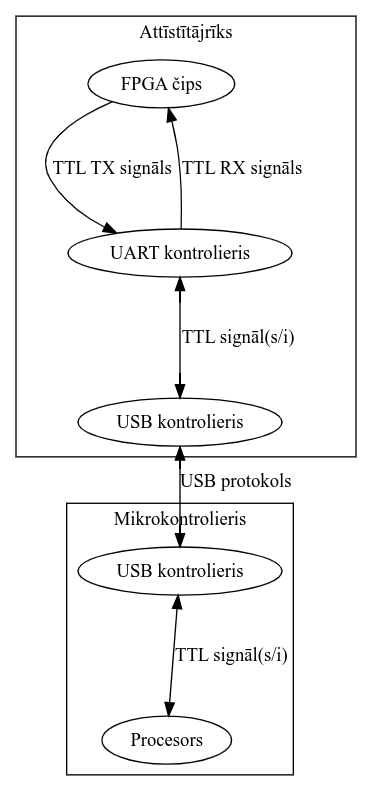
\includegraphics[width=0.3\linewidth]{assets/agentcomms-grey.png}
    \centering
    \caption{Datu apmaiņa starp attīstītājrīku un platformas "\glslink{agent}{aģentu}"}
    \label{fig:agentcomms}
\end{figure}

Ņemot vērā, šo attīstītājrīkā pieņemto komunikācijas modeli, vienīgais, ko
atliek realizēt pašam, ir projektēt \gls{ttl} seriālo komunikāciju, izmantojot
\gls{uart} mehānismu, lai nodrošinātu baitu apmaiņu starp ierīcēm. Attēlā
\ref{fig:serialframe} redzams seriālās komunikācijas kadrs iekodēts spriegumā,
ko attiecīgi var jau noprojektēt Verilog valodā, tādējādi nodrošinot
\glslink{fullduplex}{pilndupleksa} \gls{uart} baitu datu apmaiņu starp ierīcēm.
Šī darba ietvaros tika izmantota seriālā komunikācija "8-N-1" jeb ar 8 datu
bitiem, bez paritātes bita un ar vienu "stop" bitu.

\begin{figure}[H]
    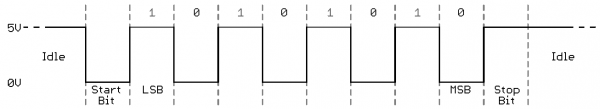
\includegraphics[width=0.7\linewidth]{assets/ttl-serial-gray.png}
    \centering
    \caption{Seriālās komunikācijas kadrs iekodēts fiziskā signālā}
    \label{fig:serialframe}
\end{figure}
